\documentclass[10pt,landscape]{article}
% next two lines required for sdsl command
\usepackage[T1]{fontenc} 
\newcommand{\changefont}[3]{\fontfamily{#1}\fontseries{#2}\fontshape{#3}\selectfont} 
\usepackage{amsfonts}

\usepackage{color}
\usepackage{multicol}
\usepackage{calc}
\usepackage{ifthen}
\usepackage[landscape]{geometry}

\usepackage{amsmath} 
\usepackage[colorlinks]{hyperref}
\usepackage{xcolor}


\usepackage{tikz}
\usepackage{endnotes} % see http://tex.stackexchange.com/questions/56145/is-there-a-way-to-move-all-footnotes-to-the-end-of-the-document
\usepackage{hyperendnotes} % see http://tex.stackexchange.com/questions/8452/making-endnotes-clickable-links-with-hyperref
\let\footnote=\endnote

\definecolor{githublink}{HTML}{4183c4}

% TODO: Add header information for classes:
%       Almost done, since abbreviations contain link to header
%

\hypersetup{
bookmarks=true,         % show bookmarks bar?
unicode=false,          % non-Latin characters in Acrobat’s bookmarks
pdftoolbar=true,        % show Acrobat’s toolbar?
pdfmenubar=true,        % show Acrobat’s menu?
pdffitwindow=false,     % window fit to page when opened
pdfstartview={FitH},    % fits the width of the page to the window
pdftitle={sdsl cheat sheet},    % title
pdfauthor={Simon Gog},     % author
pdfsubject={sdsl short reference},   % subject of the document
pdfcreator={Creator},   % creator of the document
pdfproducer={Producer}, % producer of the document
pdfkeywords={keyword1} {key2} {key3}, % list of keywords
pdfnewwindow=true,      % links in new window
colorlinks=true,       % false: boxed links; true: colored links
linkcolor=red,          % color of internal links (change box color with linkbordercolor)
citecolor=green,        % color of links to bibliography
filecolor=magenta,      % color of file links
urlcolor=githublink           % color of external links
}
% link color #4183c4
% To make this come out properly in landscape mode, do one of the following
% 1.
%  pdflatex latexsheet.tex
%
% 2.
%  latex latexsheet.tex
%  dvips -P pdf  -t landscape latexsheet.dvi
%  ps2pdf latexsheet.ps


% If you're reading this, be prepared for confusion.  Making this was
% a learning experience for me, and it shows.  Much of the placement
% was hacked in; if you make it better, let me know...


% 2008-04
% Changed page margin code to use the geometry package. Also added code for
% conditional page margins, depending on paper size. Thanks to Uwe Ziegenhagen
% for the suggestions.

% 2006-08
% Made changes based on suggestions from Gene Cooperman. <gene at ccs.neu.edu>


% To Do:
% \listoffigures \listoftables
% \setcounter{secnumdepth}{0}


% This sets page margins to .5 inch if using letter paper, and to 1cm
% if using A4 paper. (This probably isn't strictly necessary.)
% If using another size paper, use default 1cm margins.
\ifthenelse{\lengthtest { \paperwidth = 11in}}
	{ \geometry{top=.5in,left=.5in,right=.5in,bottom=.5in} }
	{\ifthenelse{ \lengthtest{ \paperwidth = 297mm}}
		{\geometry{top=1cm,left=1cm,right=1cm,bottom=1cm} }
		{\geometry{top=1cm,left=1cm,right=1cm,bottom=1cm} }
	}

% Turn off header and footer
\pagestyle{empty}
 

% Redefine section commands to use less space
\makeatletter
\renewcommand{\section}{\@startsection{section}{1}{0mm}%
                                {-1ex plus -.5ex minus -.2ex}%
                                {0.5ex plus .2ex}%x
                                {\normalfont\large\bfseries}}
\renewcommand{\subsection}{\@startsection{subsection}{2}{0mm}%
                                {-1explus -.5ex minus -.2ex}%
                                {0.5ex plus .2ex}%
                                {\normalfont\normalsize\bfseries}}
\renewcommand{\subsubsection}{\@startsection{subsubsection}{3}{0mm}%
                                {-1ex plus -.5ex minus -.2ex}%
                                {1ex plus .2ex}%
                                {\normalfont\small\bfseries}}
\makeatother

% Define BibTeX command
\def\BibTeX{{\rm B\kern-.05em{\sc i\kern-.025em b}\kern-.08em
    T\kern-.1667em\lower.7ex\hbox{E}\kern-.125emX}}

% Don't print section numbers
\setcounter{secnumdepth}{0}


\setlength{\parindent}{0pt}
\setlength{\parskip}{0pt plus 0.5ex}

% -----------------------------------------------------------------------

\DeclareMathOperator*{\argmin}{arg\!\min}

\begin{document}
\newlength{\MyLen}
\newlength{\MidLen}

\raggedright
\footnotesize
\begin{multicols}{3}


% multicol parameters
% These lengths are set only within the two main columns
%\setlength{\columnseprule}{0.25pt}
\setlength{\premulticols}{1pt}
\setlength{\postmulticols}{1pt}
\setlength{\multicolsep}{1pt}
\setlength{\columnsep}{2pt}

\newcommand{\Order}[1]{\ensuremath{{\mathcal O}(#1)}}


\newcommand{\sdslgit}{https://github.com/simongog/sdsl-lite/blob/master}
\newcommand{\sdslgitinc}{\sdslgit/include/sdsl}
\newcommand{\pizzachili}{http://pizzachili.di.unipi.it/texts.html}
\newcommand{\code}[1]{\texttt{#1}}

%\newcommand{\sdsl}{\ensuremath{\mathit{sdsl}}}
\newcommand{\sdsl}{%
{\changefont{cmss}{bx}{n}\href{\sdslgit}{sdsl}%
}%\changefont{cmr}{m}{n}%
}
%%% int vector representations
\newcommand{\sdslintvector}{\code{int\_vector}}
\newcommand{\sdslintvectorZ}{\code{int\_vector\textless\textgreater}}
\newcommand{\sdslencvector}{\code{enc\_vector}}
\newcommand{\sdslvlcvector}{\code{vlc\_vector}}
%%% coder 
\newcommand{\sdslcodereliasdelta}{\code{coder::elias\_delta}}
\newcommand{\sdslcoderfibonacci}{\code{coder::fibonacci}}
%%% bit vector representations
\newcommand{\sdslbitvector}{\code{bit\_vector}}
\newcommand{\sdslbitvectoril}{\code{bit\_vector\_il}}
\newcommand{\sdslrrrvector}{\code{rrr\_vector}}
\newcommand{\sdslsdvector}{\code{sd\_vector}}
%%%% rank support structures
\newcommand{\sdslranksupportv}{\code{rank\_support\_v}}
\newcommand{\sdslranksupportvV}{\code{rank\_support\_v5}}
\newcommand{\sdslranksupportil}{\code{rank\_support\_il}}
\newcommand{\sdslranksupportrrr}{\code{rank\_support\_rrr}}
\newcommand{\sdslranksupportsd}{\code{rank\_support\_sd}}
\newcommand{\sdslranksupportscan}{\code{rank\_support\_scan}}
%%%% select support structures
\newcommand{\sdslselectsupportmcl}{\code{select\_support\_mcl}}
\newcommand{\sdslselectsupportscan}{\code{select\_support\_scan}}
\newcommand{\sdslselectsupportil}{\code{select\_support\_il}}
\newcommand{\sdslselectsupportrrr}{\code{select\_support\_rrr}}
\newcommand{\sdslselectsupportsd}{\code{select\_support\_sd}}
%%%% WTs
\newcommand{\sdslwthuff}{\code{wt\_huff}}
\newcommand{\sdslwthutu}{\code{wt\_hutu}}
\newcommand{\sdslwtblcd}{\code{wt\_blcd}}
\newcommand{\sdslwtint}{\code{wt\_int}}
\newcommand{\sdslwtrlmn}{\code{wt\_rlmn}}
%%%% CSAs
\newcommand{\sdslcsabitcompressed}{\code{csa\_bitcompressed}}
\newcommand{\sdslcsasada}{\code{csa\_sada}}
\newcommand{\sdslcsawt}{\code{csa\_wt}}
%%%% Alphabet strategy (policy parametrization see Stroustrup C++ 24.4.1)
\newcommand{\sdslbytealphabetstrategy}{\code{byte\_alphabet}}
\newcommand{\sdslsuccinctbytealphabetstrategy}{\code{succinct\_byte\_alphabet}}
\newcommand{\sdslintalphabetstrategy}{\code{int\_alphabet}}
%%%% Alphabet strategy (policy parametrization see Stroustrup C++ 24.4.1)
\newcommand{\sdslsaordersasampling}{\code{sa\_order\_sa\_sampling}}
\newcommand{\sdsltextordersasampling}{\code{text\_order\_sa\_sampling}}

%%%% LCPs
\newcommand{\sdsllcpbitcompressed}{\code{lcp\_bitcompressed}}
\newcommand{\sdsllcpdac}{\code{lcp\_dac}}
\newcommand{\sdsllcpvlc}{\code{lcp\_vlc}}
\newcommand{\sdsllcpbyte}{\code{lcp\_byte}}
\newcommand{\sdsllcpsupportsada}{\code{lcp\_support\_sada}}
\newcommand{\sdsllcpwt}{\code{lcp\_wt}}
\newcommand{\sdsllcpsupporttree}{\code{lcp\_support\_tree}}
\newcommand{\sdsllcpsupporttreeII}{\code{lcp\_support\_tree2}}
%%%% PBSs
\newcommand{\sdslbpsupportg}{\code{bp\_support\_g}}
\newcommand{\sdslbpsupportgg}{\code{bp\_support\_gg}}
\newcommand{\sdslbpsupportsada}{\code{bp\_support\_sada}}
%%%% CSTs
\newcommand{\sdslcstsada}{\code{cst\_sada}}
\newcommand{\sdslcstsctIII}{\code{cst\_sct3}}
%%%% RMQs
\newcommand{\sdslrmqsupportsparsetable}{\code{rmq\_support\_sparse\_table}}
\newcommand{\sdslrmqsuccinctsada}{\code{rmq\_succint\_sada}}
\newcommand{\sdslrmqsuccinctsct}{\code{rmq\_succint\_sct}}

\newcommand{\myYES}{$\checkmark$}
\newcommand{\myNO}{$\times$}

\begin{center}
     \Large{\textbf{\sdsl\ Cheat Sheet}} \\
\end{center}

\section{Data structures}
The library code is in the \code{sdsl} namespace. Either import
the namespace in your program (\code{using~namespace~sdsl;}) or
qualify all identifieres by a \code{sdsl::}-prefix.

Each section corresponds to a header file. The file
is hyperlinked as part of the section heading.

We have two types of data structures in \sdsl.
\emph{Self-contained} and \emph{support}
structures. A support object \code{s} can extend
a self-contained object \code{o} (e.g. add functionality), but 
requires access to \code{o}. Support structures contain
the substring \code{support} in their class names.

\subsection{Integer Vectors (\href{\sdslgitinc/vectors.hpp}{IV})}
The core of the library is the class 
\href{\sdslgitinc/int_vector.hpp}{\sdslintvector\textless$w$\textgreater}.
Parameter $w$ corresponds to the fixed length of each
element in bits.  For $w=8,16,32,64,1$ the length is
fixed during compile time and the vectors
correspond to \href{http://www.sgi.com/tech/stl/Vector.html}{\code{std::vector\textless uint$w$\_t\textgreater}}
resp. \code{std::vector<bool>}.
If $w=0$ (default) the length can be set during runtime.
\textit{Constructor:} \sdslintvectorZ\code{($n$,$x$,$\ell$)}, with 
$n$ equals size, $x$ default integer value, $\ell$ width
of integer (has no effect for $w>0$).

\textit{Public~methods:} \code{operator[i]}, \code{size()}, \code{width()}, 
\code{data()}. 

\subsubsection{Manipulating \sdslintvector\textless$w$\textgreater\ \code{v}}
\settowidth{\MyLen}{\code{set\_random\_bits(v)}\quad}
\begin{tabular}{@{}p{\the\MyLen}%
                @{}p{\linewidth-\the\MyLen}@{}}
\textit{Method}                     & \textit{Description} \\
\code{v[$i$]=$x$}                   & Set entry \code{v[$i$]} to $x$. \\
\code{v.width($\ell$)}	            & Set width to $\ell$, if $w=0$.\\
\code{v.resize($n$)}				& Resize \code{v} to $n$ elements. \\
\multicolumn{2}{@{}l@{}}{Useful methods in namespace \code{sdsl::util}:}	\\
\code{set\_to\_value(v,$k$)} & Set \code{v[$i$]=$k$} for each $i$.\\
\code{set\_to\_id(v)}         & Set \code{v[$i$]=$i$} for each $i$.\\
\code{set\_random\_bits(v)}   & Set elements to random bits. \\
\code{mod(v,$m$)}            & Set \code{v[$i$]=v[$i$]$\bmod m$} for each $i$.\\
\code{bit\_compress(v)}       & Gets \code{$x\!=\!\max_i$v[$i$]} and 
                                      $\ell\!=\!\lceil\log(x\!-\!1)\rceil\!+\!1$  
                                      and packs the entries in $\ell$-bit integers.\\
%									  and call \code{v.width($\ell$)}.\\
\code{expand\_width(v,$\ell$)} & Expands the width of each integer to
										$\ell$ bits, if \code{$\ell\geq$~v.width().}\\
\end{tabular}

\subsubsection{Compressed Integer Vectors (\href{\sdslgitinc/vectors.hpp}{CIV})}
For a vector \code{v}, \href{\sdslgitinc/enc_vector.hpp}{\sdslencvector} stores the
self-delimiting coded deltas (\code{v[$i\!+\!1$]$-$v[$i$]}). Fast random access is
achieved by sampling values of \code{v} at rate \code{t\_dens}. Available coder
are \href{\sdslgitinc/coder_elias_delta.hpp}{\sdslcodereliasdelta} and
\href{\sdslgitinc/coder_fibonacci.hpp}{\sdslcoderfibonacci}. 

Class \href{\sdslgitinc/vlc_vector.hpp}{\sdslvlcvector} stores each
\code{v[i]} as self-delimiting codeword. Samples at rate
\code{t\_dens} are inserted for fast random access.

\subsection{Bitvectors (\href{\sdslgitinc/bit_vectors.hpp}{BV})}
Representations for a bitvector of length $n$ with $m$ set bits.
\begin{tabular}{@{}lll@{}}
\textit{Class}    & \textit{Description}       & \textit{Space}  \\
\href{\sdslgitinc/int_vector.hpp}{\sdslbitvector} & 
plain bitvector            & 64$\lceil n/64\!+\!1\rceil$ \\
\href{\sdslgitinc/bit_vector_il.hpp}{\sdslbitvectoril} &
interleaved  bitvector & $\approx n(1+K/64)$  \\
\href{\sdslgitinc/rrr_vector.hpp}{\sdslrrrvector} & 
$H_0$-compressed bitvector & $\approx \lceil \log {m\choose n} \rceil$ \\
\href{\sdslgitinc/sd_vector.hpp}{\sdslsdvector}  & sparse bitvector
& $\approx\ 2 m\cdot \log\frac{n}{m}$ \\	
\end{tabular}
\sdslbitvector\ equals \sdslintvector\code{\textless1\textgreater} and
is therefore dynamic.\\
\textit{Public Methods:} \code{operator[$i$]}, \code{size()}, \code{begin()}, \code{end()}\\
\textit{Public Types:} \code{rank\_1\_type}, \code{select\_1\_type},
                       \code{select\_0\_type}\footnote{\code{select\_0\_type} not defined for \sdslsdvector.}.
Each bitvector can be constructed out of a \sdslbitvector\ object.

\subsection{Rank Supports (\href{\sdslgitinc/rank_support.hpp}{RS})}
RSs add rank functionality to BV. Methods 
\code{rank($i$)} and \code{operator($i$)} return the number
of set bits\footnote{It is also possible to rank \code{0} or
the patterns \code{10} and \code{01}.} in the prefix $[0..i)$ of the
supported BV for $i \in [0,n]$.
\begin{tabular}{@{}llll@{}}
\textit{Class}    & \textit{Compatible BV} & \textit{+Bits} & \textit{Time} \\
\href{\sdslgitinc/rank_support_v.hpp}{\sdslranksupportv} &
\sdslbitvector & $0.25 n$ & \Order{1} \\
\href{\sdslgitinc/rank_support_v5.hpp}{\sdslranksupportvV} &
\sdslbitvector & $0.0625 n$ & \Order{1} \\
\href{\sdslgitinc/rank_support_scan.hpp}{\sdslranksupportscan} &
\sdslbitvector & 64 & \Order{n} \\
\href{\sdslgitinc/rank_support_il.hpp}{\sdslranksupportil} &
\sdslbitvectoril & 128 & \Order{1} \\
\href{\sdslgitinc/rrr_vector.hpp}{\sdslranksupportrrr} &
\sdslrrrvector & 80 & \Order{k} \\
\href{\sdslgitinc/sd_vector.hpp}{\sdslranksupportsd} &
\sdslsdvector & 64 & \Order{1} \\
\end{tabular}
Call~\code{util::init\_support(rs,bv)}~to initialize rank
structure \code{rs} to bitvector \code{bv}. Call \code{rs($i$)} to get $\code{rank(}i\code{)}=\sum_{k=0}^{k<i}\code{bv[}k\code{]}$

\subsection{Select Supports (\href{\sdslgitinc/select_support.hpp}{SLS})}\label{sec-SLS}
SLSs add select functionality to BV. Let $m$ be the number of set bits
in BV. Methods \code{select($i$)} and \code{operator($i$)} return the
position of the $i$-th set bit%
\footnote{It is also possible to select \code{0} or
the patterns \code{10} and \code{01}.}
in BV for $i\in [1..m]$.
\begin{tabular}{@{~}l@{~}l@{~~}p{9ex}l@{}}
\textit{Class}    &\textit{Compatible BV}  &\textit{+Bits}&\textit{Time}\\
\href{\sdslgitinc/select_support_mcl.hpp}{\sdslselectsupportmcl} &
\sdslbitvector & $\leq\!0.2 n$ & \Order{1}\\
\href{\sdslgitinc/select_support_scan.hpp}{\sdslselectsupportscan} &
\sdslbitvector & $64$ & \Order{n}\\
\href{\sdslgitinc/select_support_il.hpp}{\sdslselectsupportil} &
\sdslbitvectoril & $64$ & \Order{\log n}\\
\href{\sdslgitinc/rrr_select_support.hpp}{\sdslselectsupportrrr} &
\sdslrrrvector & $64$ & $\Order{\log n}$ \\
\href{\sdslgitinc/sd_select_support.hpp}{\sdslselectsupportsd} &
\sdslsdvector & $64$ & \Order{1} \\
\end{tabular}
Call~\code{util::init\_support(sls,bv)}~to initialize \code{sls} 
to bitvector \code{bv}. Call \code{sls($i$)} to get
$\code{select(}i\code{)}=\min\{j\mid \code{rank(}j\!+\!1\code{)}=i\}$. 

\subsection{Wavelet Trees (\href{\sdslgitinc/wavelet_trees.hpp}{WT}=BV+RS+SLS)}
Wavelet trees represent sequences over byte or integer alphabets of size $\sigma$ 
and consist of a tree of BVs. Rank and select on the sequences is reduced to rank and select on BVs,
and the runtime is multiplied by a factor in $[H_0,\log\sigma]$.
\begin{tabular}{@{}llcc@{}}
\textit{Class}    &\textit{Shape} & \code{lex\_ordered} & \textit{Default alphabet}\\
\href{\sdslgitinc/wt_blcd.hpp}{\sdslwtblcd} & Balanced & \myYES & byte \\
\href{\sdslgitinc/wt_huff.hpp}{\sdslwthuff} & Huffman & \myNO & byte\\
\href{\sdslgitinc/wt_hutu.hpp}{\sdslwthutu} & Hu-Tucker & \myYES & integer \\
\href{\sdslgitinc/wt_int.hpp}{\sdslwtint} & Balanced & \myYES & byte \\
\href{\sdslgitinc/wt_rlmn.hpp}{\sdslwtrlmn} & \multicolumn{3}{c}{underlying WT dependent} \\
% TODO: \verb!wt_rlg!
\end{tabular}
\textit{Public~methods:} 
\code{operator[$i$]},
\code{rank($i$,c)},
\code{select($i$,c)},
\code{inverse\_select($i$,c)},
\code{size()}, \code{begin()}, \code{end()}
\\
Order preserving WTs (\code{lex\_ordered}) provide also the 
\code{lex\_count} method. In addition
\sdslwtint\ provides: 
\code{range\_search\_2d}, 
\code{quantil\_freq},
\code{topk\_greedy},
\code{topk\_qprobing},
\code{intersect}.

\subsection{Suffix Arrays (\href{\sdslgitinc/suffix_arrays.hpp}{CSA}=IV+WT)}
Compressed suffix arrays use CIVs or WTs to represent
the suffix arrays (SA), its inverse (ISA), BWT, $\Psi$, and
LF. CSAs can be built over byte and integer alphabets. 
\begin{tabular}{@{}ll@{}}
\textit{Class}    &\textit{Description} \\
\href{\sdslgitinc/csa_bitcompressed.hpp}{\sdslcsabitcompressed} &
Based on SA and ISA stored in a IV.\\
\href{\sdslgitinc/csa_sada.hpp}{\sdslcsasada} &
Based on $\Psi$ stored in a CIV.\\
\href{\sdslgitinc/csa_wt.hpp}{\sdslcsawt} &
Based on the BWT stored in a WT.\\
\end{tabular}	
\textit{Public~methods:}
\code{operator[$i$]}, 
\code{size()},
\code{begin()},
\code{end()}.
\\
\textit{Public~members:} 
\code{isa},
\code{bwt}, 
\code{lf}, 
\code{psi}, 
\code{text}, 
\code{C}, \code{char2comp}, \code{comp2char}, \code{sigma}.\\
\textit{Policy classes: } alphabet strategy 
(e.g.
\href{\sdslgitinc/csa_alphabet_strategy.hpp}{\sdslbytealphabetstrategy},
\href{\sdslgitinc/csa_alphabet_strategy.hpp}{\sdslsuccinctbytealphabetstrategy},
\href{\sdslgitinc/csa_alphabet_strategy.hpp}{\sdslintalphabetstrategy})
and SA sampling strategy 
(e.g. 
 \href{\sdslgitinc/csa_sampling_strategy.hpp}{\sdslsaordersasampling},
 \href{\sdslgitinc/csa_sampling_strategy.hpp}{\sdsltextordersasampling}
)


\subsection{Longest Common Prefix (\href{\sdslgitinc/lcp.hpp}{LCP}) Arrays}
\begin{tabular}{@{}ll@{}}
\textit{Class}    &\textit{Description} \\
\href{\sdslgitinc/lcp_bitcompressed.hpp}{\sdsllcpbitcompressed} &
Values in a \href{\sdslgitinc/int_vector.hpp}{\sdslintvectorZ}.\\
\href{\sdslgitinc/lcp_dac.hpp}{\sdsllcpdac} &
Direct accessible codes used.\\
\href{\sdslgitinc/lcp_byte.hpp}{\sdsllcpbyte} &
Small values in a byte; 2 words per large.\\
\href{\sdslgitinc/lcp_wt.hpp}{\sdsllcpwt} &
Small values in a WT; 1 word per large.\\
\href{\sdslgitinc/lcp_vlc.hpp}{\sdsllcpvlc} &
Values in a \href{\sdslgitinc/vlc_vector.hpp}{vlc\_vector}. \\
\href{\sdslgitinc/lcp_support_sada.hpp}{\sdsllcpsupportsada} &
Values stored permuted. CSA needed. \\
\href{\sdslgitinc/lcp_support_tree.hpp}{\sdsllcpsupporttree} &
Only depths of CST inner nodes stored.\\
\href{\sdslgitinc/lcp_support_tree2.hpp}{\sdsllcpsupporttreeII} &
~+ large values are sampled using LF.\\
\end{tabular}	
\textit{Public~methods:} 
\code{operator[$i$]},
\code{size()},
\code{begin()},
\code{end()} \\

\subsection{Balanced Parentheses Supports (\href{\sdslgitinc/bp_support.hpp}{BPS})}
We represent a sequence of parentheses as a \code{bit\_vector}. 
An opening/closing parenthesis corresponds to \code{1}/\code{0}.\\
\begin{tabular}{@{}ll@{}}
\textit{Class}    &\textit{Description} \\
\href{\sdslgitinc/bp_support_g.hpp}{\sdslbpsupportg} &
Two-level pioneer structure.\\
\href{\sdslgitinc/bp_support_gg.hpp}{\sdslbpsupportgg} &
Multi-level pioneer structure.\\
\href{\sdslgitinc/bp_support_sada.hpp}{\sdslbpsupportsada} &
Min-max-tree over excess sequence.\\
\end{tabular}
\textit{Public~methods:} \code{find\_open($i$)}, \code{find\_close($i$)},
\code{enclode($i$)}, \code{double\_enclose($i$,$j$)}, \code{excess($i$)},
\code{rr\_enclose($i$,$j$)}, \code{rank($i$)}\footnote{For PBS the
bits are counted in the prefix $[0..i]$.}, \code{select($i$)}.
\\

Call~\code{util::init\_support(bps,bv)}~to initialize a BPS 
\code{bps} to \code{bit\_vector} \code{bv}. 


\subsection{Suffix Trees (\href{\sdslgitinc/suffix_trees.hpp}{CST}=CSA+LCP+BPS)}
A CST can be parametrized by any combination of CSA ,LCP, and BPS.
The operation of each part can still be accessed through member varaibles.
The additional operations are listed below.
CSTs can be built for byte or integer alphabets.
\settowidth{\MyLen}{\sdslcstsada\quad}
\begin{tabular}{@{}p{\the\MyLen}%
                @{}p{\linewidth-\the\MyLen}@{}}

\textit{Class} & \textit{Description} \\				
\href{\sdslgitinc/cst_sada.hpp}{\sdslcstsada} &
Represents a node as position in BPS. Navigational operations
are fast (they are directly translated in BPS operations on 
the DFS-BPS). Space: $4n\!+\!o(n)\!+\!|CSA|\!+\!|LCP|$ bits.\\
\href{\sdslgitinc/cst_sct3.hpp}{\sdslcstsctIII} &
Represents nodes as intervals. Fast construction, but
slower navigational operations. Space: $3n\!+\!o(n)\!+\!|CSA|\!+\!|LCP|$ \\
\end{tabular}
\textit{Public~types:} \code{node\_type}. 
In the following let $v$ and $w$ be nodes 
and $i$, $d$, $lb$, $rb$ integers.\\ 
\textit{Public~methods:} 
% CST global information
\code{nodes()},
\code{root()},
\code{begin()},
\code{end()},
\code{begin\_bottom\_up()},
\code{end\_bottom\_up},
% CST node info
\code{size($v$)},
\code{is\_leaf($v$)},
\code{degree($v$)},
\code{depth($v$)},
\code{node\_depth(v)},
\code{edge($v$, $d$)},
\code{lb($v$)},
\code{rb($v$)},
\code{id($v$)},
\code{inv\_id($i$)},
\code{sn($v$)},
% CST global navigation 
\code{select\_leaf($i$)},
\code{node($lb$, $rb$)},
% CST node navigation 
\code{parent($v$)},
\code{sibling($v$)},
\code{lca($v$, $w$)},
\code{select\_child($v$, $i$)},
\code{child($v$, $c$)},
\code{sl($v$)},
\code{wl($v$, $c$)},
\code{leftmost\_leaf($v$)},
\code{rightmost\_leaf($v$)}
\\
\textit{Public~members:} \code{csa}, \code{lcp}.\\
The \href{https://gist.github.com/simongog/5315738}{traversal example}
shows how to use the DFS-iterator.
%\textit{Iterators methods:} \code{operator++},
%\code{visit()}, \code{skip\_subtree()}   	

\subsection{Range Min/Max Query (\href{\sdslgitinc/rmq_support.hpp}{RMQ})}
A RMQ \code{rmq} can be used to determine the position of the miniumum
value\footnote{Or maximum value; can be set by a template parameter.}
in an arbitrary subrange $[i,j]$ of an preprocessed vector \code{v}.
Operator \code{operator($i$,$j$)} returns $x=\min\{$r$\mid r\in [i,j] \wedge \mbox{\code{v}[$r$]}\leq\mbox{\code{v[$k$]}}\ \forall k\in[i,j]\}$

\settowidth{\MyLen}{\sdslrmqsupportsparsetable\quad }
\settowidth{\MidLen}{$4n+o(n)$\quad}
\begin{tabular}{@{}p{\the\MyLen}%
                @{}p{\linewidth-\the\MidLen-\the\MyLen}@{}p{\the\MidLen}@{}}
\textit{Class} & \textit{Space} & \textit{Time} \\				
\href{\sdslgitinc/rmq_support_sparse_table.hpp}{\sdslrmqsupportsparsetable} &
$n \log^2 n$ & \Order{1} \\
\href{\sdslgitinc/rmq_succinct_sada.hpp}{\sdslrmqsuccinctsada} &
$4n+o(n)$    & \Order{1} \\
\href{\sdslgitinc/rmq_succinct_sct.hpp}{\sdslrmqsuccinctsct} &
$2n+o(n)$    & \Order{1} \\
\end{tabular}

\section{Constructing data structures}
Let \code{o} be a WT-, CSA-, or CST-object.
Object \code{o} is built with \code{construct(o,file,num\_bytes=$0$)}
from a sequence stored in \code{file}. File is interpreted
dependent on the value of \code{num\_bytes}:
\settowidth{\MyLen}{\code{num\_bytes=$1$}  }
\begin{tabular}{@{}p{\the\MyLen}%
                @{}p{\linewidth-\the\MyLen}@{}}
%\begin{tabular}{@{}ll@{}}
\textit{Value}      & \textit{File interpreted as}  \\
\code{num\_bytes=$0$} & serialized \code{int\_vector<>}.\\
\code{num\_bytes=$1$} & byte sequence of length \code{util::file\_size(file)}.\\
\code{num\_bytes=$2$} & 16-bit word sequence.\\
\code{num\_bytes=$4$} & 32-bit word sequence.\\
\code{num\_bytes=$8$} & 64-bit word sequence.\\	
\code{num\_bytes=d} & Parse decimal numbers.\\
\end{tabular}
Note: \code{construct} writes/reads data to/from
disk during construction. Accessing disk for small
instances is a considerable overhead. \code{construct\_im(o,data,num\_bytes=$0$)} will
build \code{o} using only main memory. Have a look
at \href{\sdslgit/tutorial/csx-printf.cpp}{this handy tool for an example}.

\subsection{Configuring construction}
The locations and names of the intermediate files
can be configured by a \code{cache\_config} object.
It is constructed by 
\code{cache\_config(del,tmp\_dir,id, map)}
where
\code{del} is a boolean variable which specifies
if the intermediate files should be deleted after construction,
\code{tmp\_dir} is a path to the directory where
the intermediate files should be stored,
\code{id} is used as part of the file names,
and \code{map} contains a mapping of keys
(e.g. \href{\sdslgitinc/config.hpp}{\code{conf::KEY\_BWT}}, 
      \href{\sdslgitinc/config.hpp}{\code{conf::KEY\_SA}},\ldots)
to file paths.\\
The \code{cache\_config} parameter extends the construction method to:
\code{construct(o,file,config,num\_bytes)}.\\
The following methods (\code{key} is a key string, \code{config} represenet a  
\code{cache\_config} object, and \code{o} a \sdsl\ object) should be handy
in customized construction processes:\\
\code{cache\_file\_name(key,config)}\\
\code{cache\_file\_exists(key,config)}\\
\code{register\_cache\_file(key,config)}\\
\code{load\_from\_cache(o,key,config)}\\
\code{store\_to\_cache(o,key,config)}\\

\subsection{Resource requirements}
\textit{Memory}: The memory peak of CSA and CST construction occurs during the SA
construction, which is $5$ times the texts size for byte-alphabets
and inputs $<2$ GiB (see the Figure below for a $200$ MB text) 
and $9$ times for larger inputs. For integer
alphabets the construction takes about twice the space of
the resulting output.\\
\textit{Time}: A CST construction processes at about $2\mbox{ MB}/s$.
The Figure below shows the resource consumption during the construction
of a \code{cst\_sct3<>} CST for \href{\pizzachili}{$200$ MB English text}.
For a detailed description of the phases click on the figure.
\href{http://simongog.github.io/assets/data/cst-construction.html}{%
\scalebox{0.18}{%
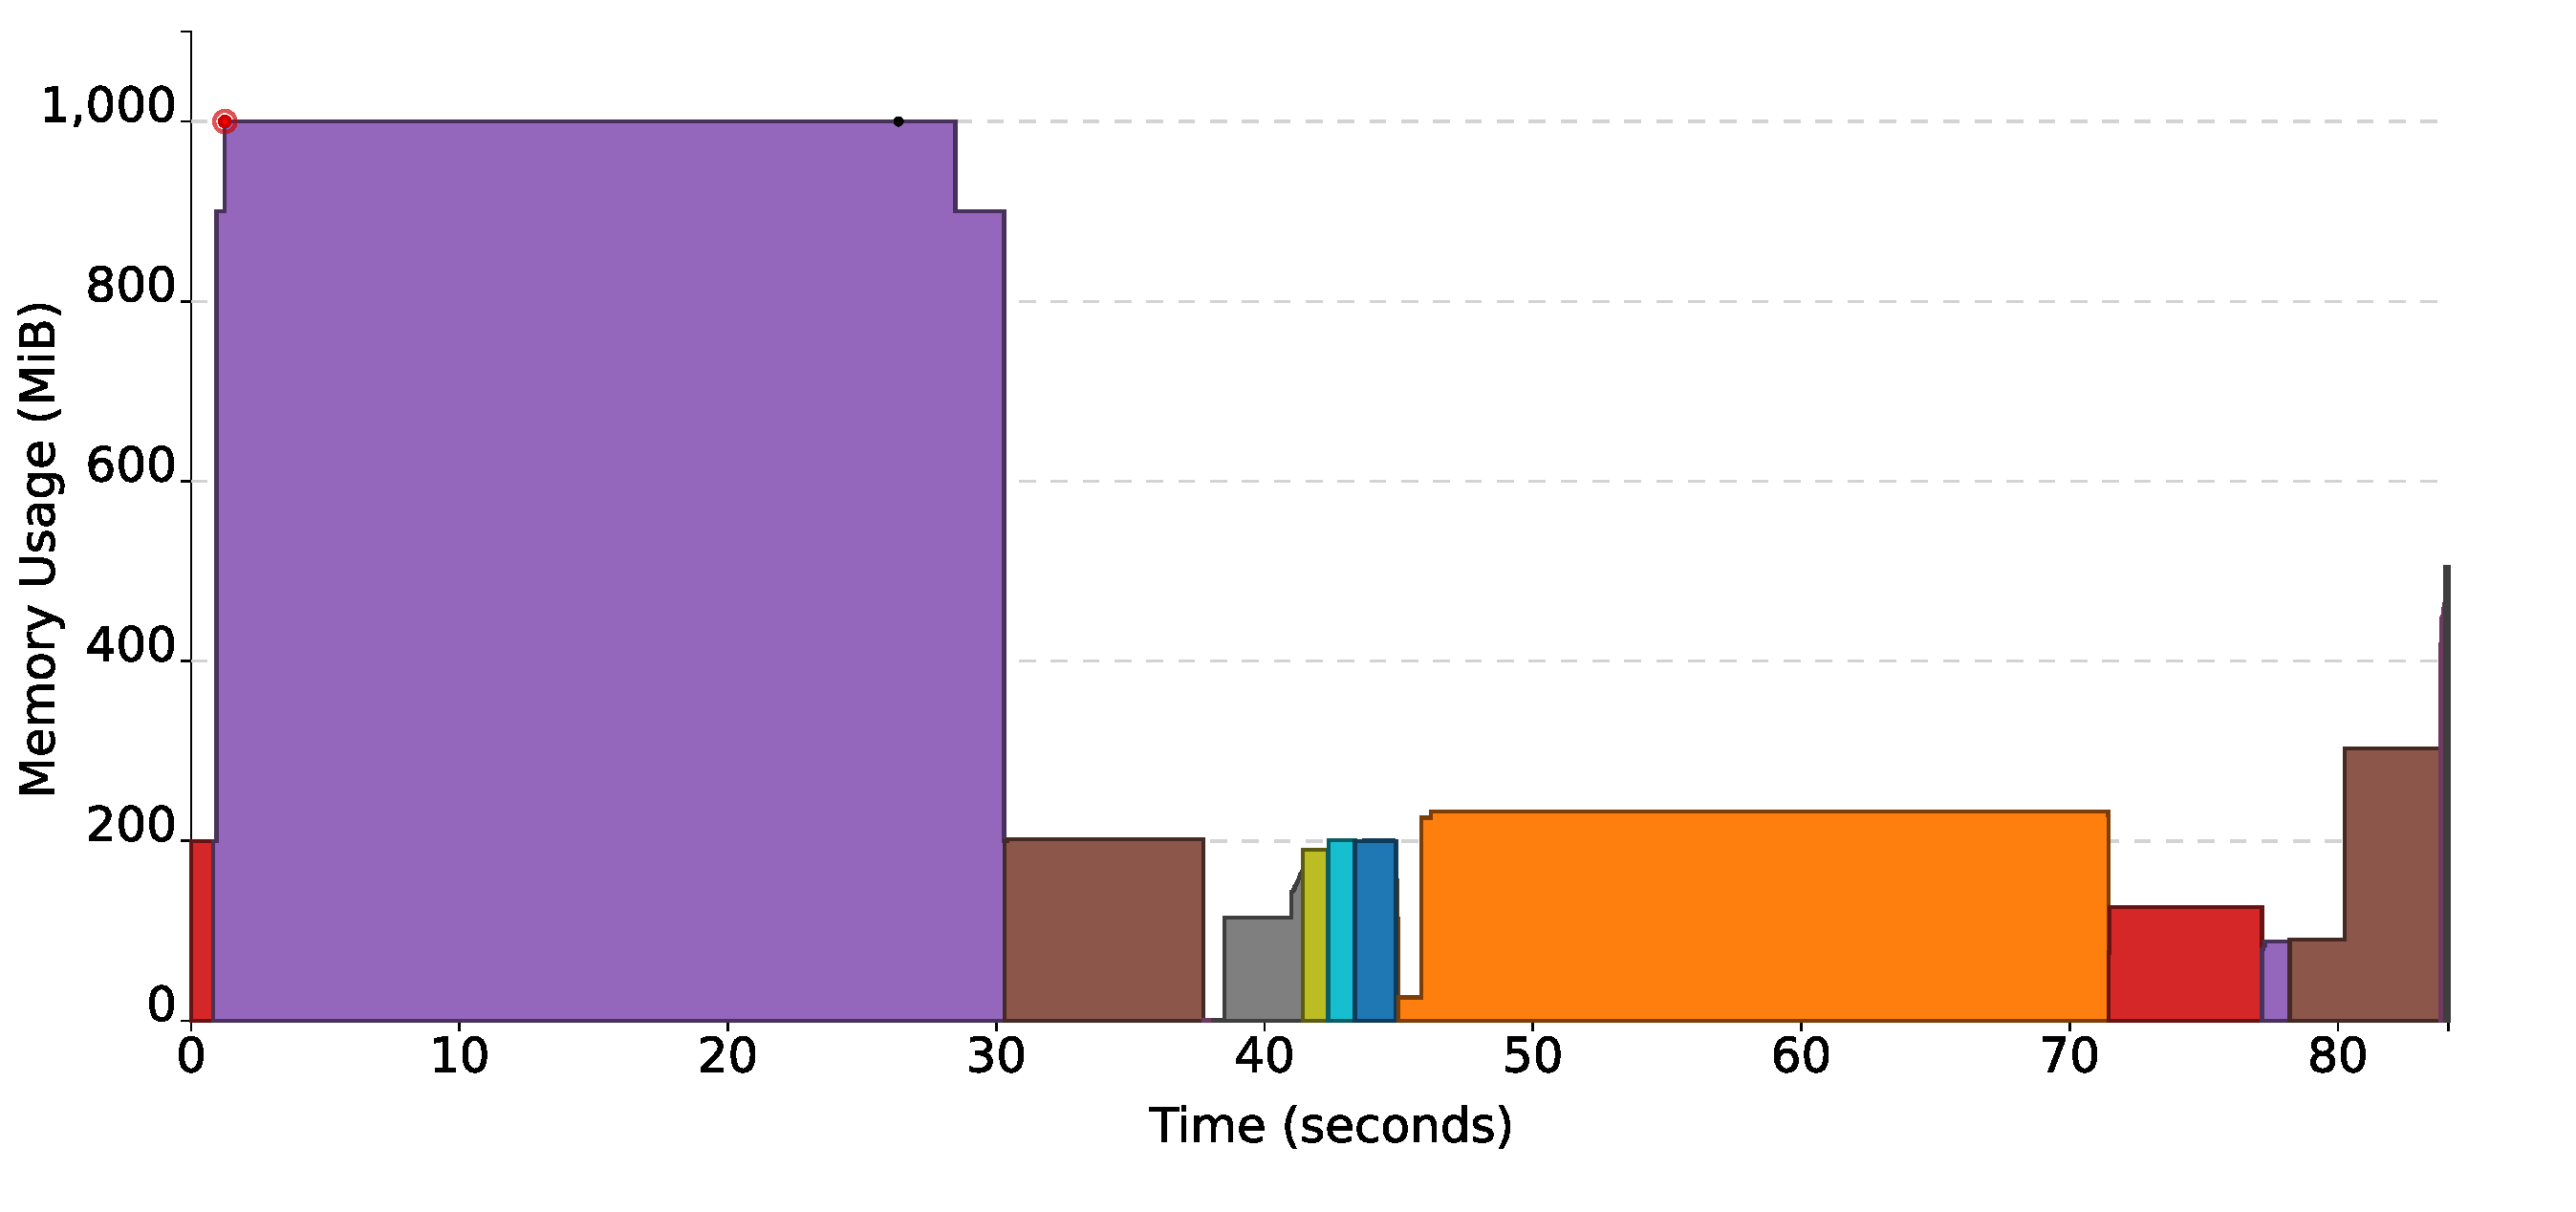
\includegraphics{viz.pdf}%
}%
}
This diagram was generated using the sample program
\href{\sdslgit/tutorial/memory-visualization.cpp}{memory-visualization.x},

\section{Reading and writing data}
\subsection{Importing data into \sdsl\ structures}
\begin{tabular}{@{}p{0.9\linewidth}@{}}
\code{load\_vector\_from\_file(v, file, num\_bytes)} \\
Load \code{file} into an \code{int\_vector}~\code{v}. Interpretation
of \code{file} depends on \code{num\_bytes}; see method \code{construct}.
\end{tabular}
%TODO: mention io wrappers


\subsection{Store \sdsl\ structures}
Use \code{store\_to\_file(o, file)} 
to store an \sdsl\ object \code{o} to \code{file}.
Object \code{o} can also be serialized
into a \code{std::ostream}-object \code{out}
by the call \code{o.serialize(out)}.

%\code{write\_member($x$,out)}
%\code{read\_member($x$,in)}

\subsection{Load \sdsl\ structures}
Use \code{load\_from\_file(o, file)} to load 
an \sdsl\ object \code{o}, which is stored in \code{file}. 
Call \code{o.load(in)} reads \code{o} from
\code{std::istream}-object \code{in}.

%TODO: mention io wrappers

\section{Utility methods}
More useful methods in the \code{sdsl::util} namespace:


\settowidth{\MyLen}{\code{assign(t1,t2)}~}
\begin{tabular}{@{}p{\the\MyLen}%
                @{}p{\linewidth-\the\MyLen}@{}}
%\begin{tabular}{@{}ll@{}}
\textit{Method}      & \textit{Description}  \\
\code{pid()}         & Id of current process. \\
\code{id()}          & Get unique id inside the process. \\
\code{basename(p)}   & Get filename part of a path \code{p}.  \\
\code{dirname(p)}    & Get directory part of a path \code{p}. \\
\code{demangle(o)}   & Demangles output of \code{typeid(o).name()}.\\
\code{demangle2(o)}  & Simplifies output of \code{demangle}. E.g. removes \code{sdsl::}-prefixes, \ldots \\
\code{to\_string(o)} & Transform object \code{o} to a string. \\
\code{assign(o1,o2)} & Assign \code{o1} to \code{o2}, or swap \code{o1} and \code{o2} if
                       the objects are of the same type.\\
\code{clear(o)}      & Set o to the empty object.\\
%\code{swap\_support(s1, s2, t1, t2)}\\
\end{tabular}

\section{Measuring and Visualizing Space}
\code{size\_in\_bytes(o)} returns the space used by an
\sdsl\ object \code{o}. Call
\code{write\_structure<JSON\_FORMAT>(o,out)} to get
a detailed space breakdown written in 
\href{http://www.json.org/}{JSON} format to stream \code{out}.
\code{<HTML\_FORMAT>} will write a HTML page
(\href{http://simongog.github.io/assets/data/space-vis.html}{like this}),
which includes an interactive SVG-figure.


\section{Methods on words}
Class \code{bits} contains various fast methods
on a $64$-bit word $x$. Here the most important ones.
\settowidth{\MyLen}{\code{bits::sel($x$, $i$)}~}
\begin{tabular}{@{}p{\the\MyLen}%
                @{}p{\linewidth-\the\MyLen}@{}}
%\begin{tabular}{@{}ll@{}}
\textit{Method}      & \textit{Description}  \\
\code{bits::cnt($x$)}  & Number of set bits in $x$.\\
\code{bits::sel($x$,$i$)}& Position of $i$-th set bit, $i\in[0,\code{cnt($x$)}\!-\!1)$. \\
\code{bits::lo($x$)}   & Position of least significant set bit.\\
\code{bits::hi($x$)}   & Position of most significant set bit.\\
\end{tabular}
\textit{Note}: Positions in $x$ start at $0$.
\code{lo} and \code{hi} return $0$ for $x=0$.

\section{Tests}
A \code{make test} call in the \href{\sdslgit/test}{test}
directory, downloads test inputs, compiles tests,
and executes them.

\section{Benchmarks}
Directory \href{\sdslgit/benachmark}{benchmark}
contains configurable benchmarks for various
data structure, like CSAs/FM-indexes (measuring
time and space for operations 
\href{\sdslgit/benchmark/indexing_count}{count},
\href{\sdslgit/benchmark/indexing_locate}{locate}, and
\href{\sdslgit/benchmark/indexing_extract}{extract}).

\section{Debugging}
You get the gdb command \code{pv <int\_vector> <idx1> <idx2>},
which displays the elements of an \sdslintvector\ in the
range $[\code{idx1},\code{idx2}]$ by appending  the file
\href{\sdslgit/extras/sdsl.gdb}{sdsl.gdb} to your
\code{.gdbinit}. 

%\section{Acknowledgements}
%Yuta Mori for implementing libdivsufsort, which
%is used to construct SAs.
%
%Jesper Larsson for integer-alphabet SA construction.
%
\rule{0.3\linewidth}{0.25pt}
\scriptsize

\copyright\ Simon Gog

Cheatsheet template provided by Winston Chang
http://www.stdout.org/$\sim$winston/latex/

\theendnotes

\end{multicols}
%\newpage
%~
\end{document}
